\section{Knowledge Graph Construction with Declarative Mapping Rules \textcolor{red}{By 12/1}}
\label{sec:chp2_declarative_kgc}

Knowledge graphs can be constructed in diverse manners. One way comprises collecting knowledge from contributions form the community, such as Wikidata. Other way involves transforming data from heterogeneous formats and sources, unstructured or (semi-)structured, into RDF. This section focuses on providing an overview of the latter, to declaratively construct knowledge graphs from heterogeneous data sources.

%\ana{overview de distintas formas y métodos en general de construir KGs. Debería ser algo larga, ampliando lo que hay en la intro. Luego terminar con enfocarse en los approaches declarativos, que se extienden en la siguiente subsección}

%\ana{RAW} In this section, the current scene of mapping languages is described first, regardless of the approach they follow, i.e., RDF materialization or virtualization. Then, previous works comparing mapping languages are surveyed. 


Constructing RDF knowledge graphs from heterogeneous data sources involve a schema transformation of the data to the desired graph structure. This transformation may be done in several different ways, usually involving mapping languages that allow expressing the transformation rules to create the target graphs. Hence, these mappings hold declaratively the relationships between the source and target data schemas. This comprises an agnostic approach that can (and has been) applied to multiple different use cases. \ana{refs}

The usual workflow in which declarative approaches are involved is depicted in \ana{figure}. They enable both materialization and virtualization of knowledge graphs. In materialization scenarios, data is transformed into the target graph, usually following the schema provided by an ontology. In virtualization scenarios, data is not transformed; instead, the original data source is accessed also following the schema of the target (virtual) graph. This process requires translating the original query into the language of the original data source. \ana{mention OBDA?}

This section presents an overview of existing mapping languages.  We first show two RDF-based mapping languages that have had a significant impact, the W3C Recommendation R2RML (\cref{sec:chp2_R2RML}), and its most impactful extension, RML (\cref{sec:chp2_RML}); and then other relevant languages (\cref{sec:chp2_more-languages}). Lastly, we discuss the approaches that compare the diversity and expressiveness of these mapping languages (\cref{sec:chp2_language-comparison}).






\subsection{R2RML: RDB to RDF Mapping Language}
\label{sec:chp2_R2RML}

R2RML~\parencite{das2012r2rml} addresses the transformation of data in relational databases into RDF. This language specifies to write the transformation rules in R2RML mapping documents. An R2RML mapping document is composed by at least one \textit{Triples Map} (\texttt{rr:TriplesMap}). \textit{Triples Maps} are used to define the transformation rules to generate RDF triples, and contain:

\begin{itemize}
    \item One \textit{Logical Table} (\texttt{rr:LogicalTable}), that describes the source relational table or view of a database.
    \item One \textit{Subject Map} (\texttt{rr:SubjectMap}), that defines how to generate the subject of the triples, and optionally, the corresponding class(es) it may be instance of (\texttt{rr:class}).
    \item Zero to multiple \textit{Predicate-Object Maps} (\texttt{rr:PredicateObjectMap}). A \textit{Predicate-Object Map} (POM) is formed by one to multiple \textit{Predicate Maps} (\texttt{rr:PredicateMap}), and one to many \textit{Object Maps} (\texttt{rr:ObjectMap}).% or \textit{Referencing Object Maps} (\texttt{rr:RefObjectMap}). The former is used for regular objects of triples, and the latter for creating as object the subject of another \textit{Triples Map}. 
\end{itemize}

Zero or more \textit{Graph Maps} (\texttt{rr:GraphMap}), which indicate how to generate named graphs, can be assigned to both \textit{Subject Maps} and \textit{Predicate Object Maps}. 
It is also possible to join \textit{Logical Tables} by replacing \textit{Object Map} by \texttt{Referencing Object Maps} (\texttt{rr:RefObjectMap}), which uses the subject of another \textit{Triples Map}, indicated with \texttt{rr:parentTriplesMap}, as the object of the triple. 
This join may have a condition to be performed, which is indicated using \texttt{rr:joinCondition}, \texttt{rr:child}, and \texttt{rr:parent}. 
Additionally, \textit{Object Maps} may include additional information, such as datatypes (\texttt{rr:datatype}) and languages (\texttt{rr:language}) of literals. \ana{figure of triples map}

\textit{Subject Map}, \textit{Predicate Map}, \textit{Object Map}, and \textit{Graph Map} are subclasses of \textit{Term Map} (\texttt{rr:TermMap}), which define how to generate RDF terms. 
\textit{Term Maps} can be (i) \textit{constant-valued} (\texttt{rr:constant}), i.e., always generating the same RDF term; 
(ii) \textit{column-valued} (\texttt{rr:column}), i.e., the RDF terms are directly obtained from cells of a column in the RDB; 
or (iii) \textit{template-valued} (\texttt{rr:template}), i.e., the RDF terms are composed from the data in columns and constant strings. These terms can be generated either as IRIs (\texttt{rr:IRI}), Blank Nodes (\texttt{rr:BlankNode}) or literals (\texttt{rr:Literal}) using \texttt{rr:termType}.  \ana{figure of term map}

\ana{example}

\subsection{RML: RDF Mapping Language}
\label{sec:chp2_RML}
RML~\parencite{Dimou2014rml} extends R2RML to address the transformation of heterogeneous data formats, such as CSV, XML or JSON. Broadening the possibilities for KG construction with minimal changes in the vocabulary with respect to the standard, this language rapidly gained importance, and currently gathers an active community of users and developers. 

The main differences of RML with R2RML~\parencite{dimou2020rml-r2rml-diffs} are listed as follows:
\begin{itemize}
    \item \textbf{Data source reference}. RML introduces the \textit{Logical Source} (\texttt{rml:LogicalSource}), that extends R2RML's \textit{Logical Table}. Where the \textit{Logical Table} focuses on relational databases, the \textit{Logical source} enables the description of more heterogeneous data sources in addition to relational databases.

    \item \textbf{Data source language}. In R2RML, the data source language is implicitly assumed to be SQL. To address heterogeneous data formats, RML uses the \textit{Reference Formulation} (\texttt{rml:ReferenceFormulation}) to indicate which formulation is suitable to parse data in a specific format. For instance, the JSONPath formation can be used for parsing data in a JSON file. 

    \item \textbf{Iteration}. For tabular data sources, the iteration of the data source is per row. This strategy is followed by every R2RML processor to construct RDF graphs from RDBs. For non-tabular data sources, the iteration cannot always be implicitly assumed. For this reason, RML introduces the \textit{Iterator} (\texttt{rml:iterator})enabling the explicit determination of the iteration pattern to specify the specific data used in each iteration to build the RDF triples. The use of the \textit{Iterator} is optional, its use relies on the needs and particularities of each data source and use case.

    \item \textbf{Value reference}. R2RML relies on column names when referring to values in a table or view of a RDB (\texttt{rr:column}). RML broadens the scope of this concept using \textit{References} (\texttt{rml:reference}), that may refer to columns, objects (such as in the case of XML and JSON) or other elements valid with respect to the used \textit{Reference Formulation}. 
\end{itemize}

\ana{example}

Several proposals have been proposed for RML in the following years of its release to extend its capabilites. The initial features for addressing heterogeneous data sources were expanded by~\cite{}~\ana{ref de 2015}, allowing more diverse data accesses and fine-grained description of the data sources. RML+FnO \cite{DeMeester2017fno_dbpedia}. \cite{delva2021rml-fields} introduced the RML Fields, that allowed [+++]. RML spreadsheets (markus). RML Target by \cite{VanAssche2021LeveragingWebThings}. RDF-star by \cite{delva2021rml-star}. 

The Knowledge Graph Construction W3C Community Group has gathered these variety of specifications and released a new version of RML~\parencite{iglesias2023rml}, that includes several of these extensions, overcoming the identified limitations for declarative KG construction.




\subsection{Additional Mapping Languages}
\label{sec:chp2_more-languages}

Following, we present an overview of existing mapping languages, listed in \cref{tab:chp2_languages_summary} and depicted in  \cref{fig:chp2_mapping_languages}. This section presents additional relevant languages classified in three categories, based on the schema they are based on or extend: (i)~RDF-based (\cref{sec:chp2_RDF-languages}), (ii)~SPARQL-based (\cref{sec:chp2_SPARQL-languages}), and (iii)~based on alternative schemas (\cref{sec:chp2_alternative-languages}).


\begin{table}[t]
\caption[Mapping languages overview]{Analyzed mapping languages and their corresponding references.}
\label{tab:chp2_languages_summary}
\resizebox{\columnwidth}{!}{
\begin{tabular}{ccc}
%\rowcolor[HTML]{EFEFEF} 
\textbf{Classification}                 & \textbf{Language}        & \textbf{Reference(s)} \\ \midrule
\multirow{15}{*}{\textbf{RDF-based}}   & D2RQ            & \parencite{bizer2004d2rq,d2rq}\\ \cmidrule{2-3} 
                              & R$_2$O          & \parencite{barrasa2004r2o}\\ \cmidrule{2-3} 
                              & R2RML           & \parencite{das2012r2rml}\\ \cmidrule{2-3} 
                              & xR2RML          & \parencite{michel2015xr2rml,xr2rml}\\ \cmidrule{2-3} 
                              & RML             & \parencite{Dimou2014rml,rml}\\ \cmidrule{2-3} 
                              & KR2RML          & \parencite{slepicka2015kr2rml}\\ \cmidrule{2-3} 
                              & FunUL           & \parencite{junior2016funul}\\ \cmidrule{2-3} 
                              & R2RML-F         & \parencite{debruyne2016r2rmlf}\\ \cmidrule{2-3} 
                              & D2RML           & \parencite{chortaras2018d2rml}\\ \cmidrule{2-3} 
                              & R2RML for collections & \parencite{debruyne2017R2RML-collections}\\ \cmidrule{2-3}   
                              & XLWrap          & \parencite{langegger2009xlwrap,xlwrap}\\ \cmidrule{2-3} 
                              & CSVW            & \parencite{Tennison2015csvw}\\ \midrule
\multirow{6}{*}{\textbf{SPARQL-based}} & SPARQL-Generate &     
                              \parencite{Lefrancois2017sparqlgenerate,sparqlgenerate}\\ \cmidrule{2-3} 
                              & XSPARQL         & \parencite{Bischof2012xsparql,xsparql}\\ \cmidrule{2-3} 
                              & TARQL           & \parencite{tarql}\\ \cmidrule{2-3}
                              & Facade-X        & \parencite{asprino2023sparql-anything,sparqlanything}\\ \cmidrule{2-3}
                              & Sansa            & \parencite{stadler2023spark}\\ \midrule
\multirow{4}{*}{\textbf{Alternative schema}}       & Helio mappings  & \parencite{cimmino2022helio}\\ \cmidrule{2-3} 
                              & D-REPR          & \parencite{Vu2019d-repr}\\ \cmidrule{2-3} 
                              & ShExML          & \parencite{Garcia-Gonzalez2020shexml,shexml}\\  \bottomrule
\end{tabular}}
\end{table}



\begin{figure*}[t]
\centering
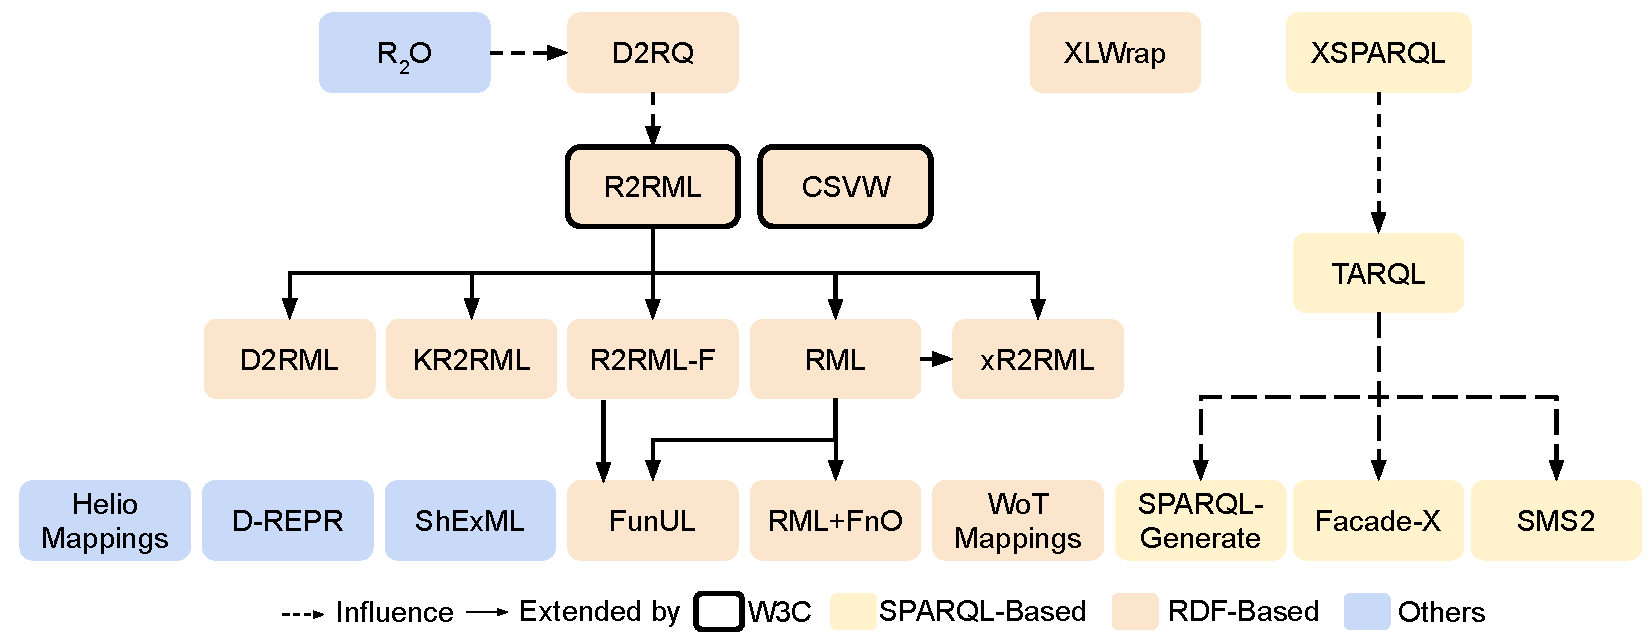
\includegraphics[width=1\linewidth]{figures/chp2_mapping_languages}
\caption[Existing mapping languages and the relationships among them]{Mapping languages developed in the last two decades, classified according to the schema they are based on, and the relationships among them.}
\label{fig:chp2_mapping_languages}
\end{figure*}

\subsubsection{RDF-based mapping languages.} 
\label{sec:chp2_RDF-languages}

Mapping languages in this group are formalized using RDF. They are usually modelled as ontologies or vocabularies that enable the description of data transformation rules. Mappings that follow these languages are usually written in files following the Turtle syntax~\parencite{turtle}. R2RML and RML, previously presented in \cref{sec:chp2_R2RML}
and \cref{sec:chp2_RML} respectively, also belong to this group of languages. 


\noindent\textbf{D2RQ}~\parencite{bizer2004d2rq} One of the first mapping languages, developed to access the content of non RDF relational databases. 

\noindent\textbf{XLWrap}~\parencite{langegger2009xlwrap}

\noindent\textbf{KR2RML}~\parencite{slepicka2015kr2rml}

\noindent\textbf{xR2RML}~\parencite{michel2015xr2rml}

\noindent\textbf{FunUL}~\parencite{junior2016funul}

\noindent\textbf{R2RML-F}~\parencite{debruyne2016r2rmlf}

\noindent\textbf{R2RML for collections and containers}~\parencite{debruyne2017R2RML-collections}

\noindent\textbf{D2RML}~\parencite{chortaras2018d2rml}

\noindent\textbf{CSVW}~\parencite{Tennison2015csvw}

\textit{The most well-known language in this category is R2RML~\parencite{das2012r2rml}, which allows mapping of data stored in relational databases to RDF. This language is heavily influenced by previous languages (R$_2$O~\parencite{barrasa2004r2o} and D2RQ~\parencite{bizer2004d2rq}). Some serializations (e.g. SML~\parencite{Stadler2015sml}, OBDA mappings from Ontop~\parencite{rodriguez2015efficient}) and several extensions of R2RML were developed in the following years after its release: R2RML-f~\parencite{debruyne2016r2rmlf} extends R2RML to include functions to be applied over the data; RML~\parencite{Dimou2014rml} and its user-friendly compact syntax YARRRML~\parencite{Heyvaert2018yarrrml} provide the possibility of covering additional data formats (CSV, XML and JSON); this language also considers the use of functions for data transformation (e.g. lowercase, replace, trim) by using the Function Ontology (FnO)\footnote{\url{https://fno.io/rml/}}~\parencite{DeMeester2017fno_dbpedia}; FunUL~\parencite{junior2016funul} proposes an extension to also incorporate functions, but focusing on the CSV format; KR2RML~\parencite{slepicka2015kr2rml} is also an extension for CSV, XML and JSON, with the addition of representing all sources with the Nested Relational Model as an intermediate model and the possibility of cleaning data with Python functions; xR2RML~\parencite{michel2015xr2rml} extends R2RML and RML to include NoSQL databases and incorporates more features to handle tree-like data; D2RML~\parencite{chortaras2018d2rml}, also based on R2RML and RML, is able to transform data from XML, JSON, CSVs and REST/SPARQL endpoints, and enables functions and conditions to create triples. }

\textit{In this category, we can also find more languages not related to R2RML. XLWrap~\parencite{langegger2009xlwrap} is focused on transforming spreadsheets into different formats. CSVW~\parencite{Tennison2015csvw} enables tabular data annotation on the Web with metadata, but also supports the generation of RDF. Finally, WoT Mappings~\parencite{cimmino2020ewot} are oriented to be used in the context of the Web of Things.}




\subsubsection{SPARQL-based mapping languages.}
\label{sec:chp2_SPARQL-languages} 

This group is integrated by languages that leverage the SPARQL query language, usually by extending its features to describe non-RDF data sources~\parencite{harris2013sparql}. 


\noindent\textbf{XSPARQL}~\parencite{Bischof2012xsparql}

\noindent\textbf{SPARQL-Generate}~\parencite{Lefrancois2017sparqlgenerate}

\noindent\textbf{TARQL}~\parencite{tarql}

\noindent\textbf{SPARQL-Anything}~\parencite{asprino2023sparql-anything}

\noindent\textbf{Sansa/whatever}~\parencite{stadler2023spark}




\textit{XSPARQL~\parencite{Bischof2012xsparql} merges SPARQL and XQuery to transform XML into RDF. TARQL~\parencite{tarql} uses the SPARQL syntax to generate RDF from CSV files. SPARQL-Generate~\parencite{Lefrancois2017sparqlgenerate} is capable of generating RDF and document streams from a wide variety of data formats and access protocols. Most recently, Facade-X has been developed, not as a new language, but as a "\textit{facade} to wrap the original resource and to make it queryable as if it was RDF"~\parencite{asprino2023sparql-anything}. It does not extend the SPARQL language, instead it overrides the SERVICE operator. Lastly, authors would like to highlight a loosely SPARQL-based language, Stardog Mapping Syntax 2 (SMS2)~\parencite{sms2}, which represents virtual Stardog graphs and is able to support sources such as JSON, CSV, RDB, MongoDB and Elasticsearch.}




\subsubsection{Based on alternative schemas.} 
\label{sec:chp2_alternative-languages}

Lastly, the languages of this group rely on schemas different from RDF or SPARQL, equally able and expressive enough to enable users to write transformation rules. 


\noindent\textbf{R$_2$O}~\parencite{barrasa2004r2o} XML-based~\footnote{https://pdfs.semanticscholar.org/4c47/0826aafc07fc6d37ca7e2474c1d3b290ade1.pdf}

\noindent\textbf{D-REPR}~\parencite{Vu2019d-repr}

\noindent\textbf{ShExML}~\parencite{Garcia-Gonzalez2020shexml,garcia2021shexml-challenges}

\noindent\textbf{Helio??}~\parencite{cimmino2022helio}

\textit{ShExML~\parencite{Garcia-Gonzalez2020shexml,garcia2021shexml-challenges} uses Shape Expressions (ShEx)~\parencite{prud2014shex} to map data sources in RDBs, CSV, JSON, XML and RDF using SPARQL queries. The Helio mapping language~\parencite{cimmino2022helio} is based on JSON and provides the capability of using functions for data transformation and data linking~\parencite{cimmino2018hybrid}. D-REPR~\parencite{Vu2019d-repr} focuses on describing heterogeneous data with JSONPath and allows the use of data transformation functions. XRM (Expressive RDF Mapper)~\parencite{xrm} is a commercial language that provides a unique user-friendly syntax to create mappings in R2RML, CSVW and RML.}










\subsection{Mapping Languages Comparison}
\label{sec:chp2_language-comparison}

As the number of mapping languages increased and their adoption grew wider, comparisons between these languages inevitably occurred. This is the case of, for instance, SPARQL-Generate~\parencite{Lefrancois2017sparqlgenerate}, which is compared to RML in terms of query/mapping complexity; and ShExML~\parencite{Garcia-Gonzalez2020shexml}, which is compared to SPARQL-Generate and YARRRML from a usability perspective.

Some studies dig deeper, providing qualitative complex comparison frameworks. Hert et al.~\parencite{hert2011comparison} provide a comparison framework for mapping languages focused on transforming relational databases to RDF. The framework is composed of 15 features, and the languages are evaluated based on the presence or absence of these features.% (Logical table to class, M:N relationships, project attributes, select conditions, user-defined instance URIs, literal to URIs, vocabulary reuse, transformation functions, datatypes, named graphs, blank nodes, integrity constraints, static metadata, one table to \textit{n} classes, and write support). 
The results lead authors to divide the mappings into four categories (direct mapping, read-only general-purpose mapping, read-write general-purpose mapping, and special-purpose mapping), and ponder on the heavy reliance of most languages on SQL to implement the mapping, and the usefulness of read-write mappings (i.e., mappings able to write data in the database). De Meester et al.~\parencite{DeMeester2019comparison} show an initial analysis of 5 similar languages (RML+FnO, xR2RML, FunUL, SPARQL-Generate, YARRRML) discussing their characteristics, according to three categories: non-functional, functional and data source support. The study concludes by remarking on the need to build a more complete and precise comparative framework and asking for a more active participation from the community to build it. To the best of our knowledge, there is no comprehensive work in the literature comparing all existing languages. \ana{ojo con esto que con el survey de ghent ya no es del todo cierto :(} 
